\chapter{Experiment}
\label{ch:Experiment}
As has already been shown, the sealing of valves is essential for the reliability of 
pipeline transport in hydraulic and pneumatic systems. Leakage can impact the efficiency
 of industrial production and contribute to the occurrence of potential dangers. 
Due to these factors, it is crucial to investigate leaks in metal valves. According to a search 
of the scholarly literature, there are limited discussions of the effect of particles in fluids 
and their concentration on the sealability of metal valves. For the investigation of these 
factors' effects on the sealing of metal valves, the improvement of the test rig and the 
reasonable assessment of leakage under varying experimental settings are therefore imperative.

\section{Test Rig}
\label{Test Rig}
Figure \Ref{fig:TestRig1} depicts a developed experimental platform that was available before this study 
was carried out. A ball seat valve, a water tank, pipelines, an air motor, a hydraulic pump,
and ball valves are its primary components. The medium passing through the pipeline 
consists of distilled water and various types of microscopic particles. Distilled water
was chosen for two primary reasons. First, it comprises a negligible amount of particles,
which has the least potential impact on the particles being analyzed and reduces the 
errors caused in the test results. Also, water has a smaller viscosity as compared to
hydraulic oil, which is usually used in industrial applications. 
The smaller viscosity leads to a higher leakage, which is easier to measure \cite{fischer2021influence}.\\

\begin{figure}[htbp]
    \centering
    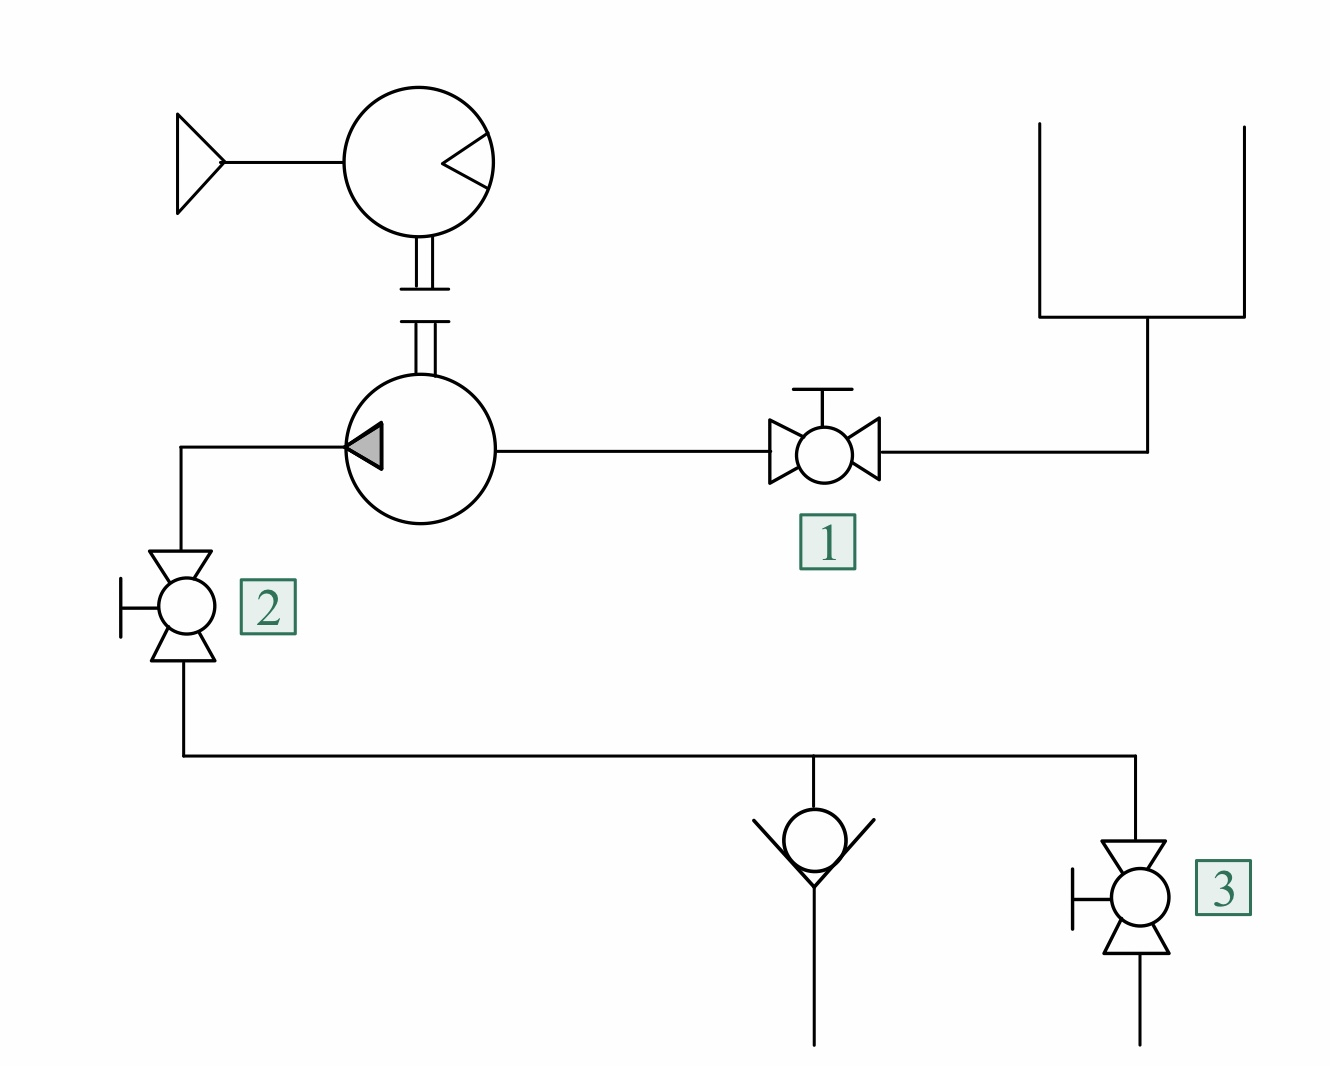
\includegraphics[width=0.5\textwidth]{figures/TestRig/TestRig1.jpg}
    \caption{Sketch of a original available test rig.}
    \label{fig:TestRig1}
\end{figure}

Distilled water and particles will be mixed in a specific proportion. 
Through the water tank, the mixture is pumped into the pipeline, where 
it is transformed into a hydraulic medium and delivered on to the valve. 
Due to the imperfect sealing of the ball seat valve, distilled water can leak 
from a high-pressure environment to a low-pressure environment, i.e., to the 
atmosphere where the relative pressure is zero. This facilitates the detection of leaks, 
and the sealing of the ball seat valve can be analyzed by measuring the amount of leakage.\\

The initial testing platform will be upgraded in order to keep the distilled water and microscopic
 particles in the pipeline as uniformly mixed as feasible. As illustrated in Figure \Ref{fig:TestRig1}, 
 the medium 
 entering the pipe from the tank either leaks into the atmosphere through the valve or flows out as 
 wastewater at the end of the experiment through the opened drain ball valve No. 3 at the pipe's end, 
 indicating that the pipe is not a closed circuit. During the process of measuring the leakage of the 
 ball seat valve, the No. 3 drain valve always remains closed. When the sealing of the ball seat valve 
 is not particularly poor, the amount of leaking fluid will be small, resulting in the mixture entering 
 the pipe only being dynamic when it is just flowing into the pipe. As the mixture fills the pipe, its 
 state gradually becomes static, which is likely to cause tiny particles to settle downwards due to their
  own weight, thus accumulating in the pipe and failing to mix evenly with the distilled water, resulting 
  in the actual concentration of particles in the mixture passing through the ball seat valve 
 deviating too greatly from the initial set concentration added to the water tank.\\

 The test rig was improved by connecting the end of the original pipe to the tank with a new section of
  pipe and a ball valve No. 4, as illustrated in Figure \Ref{fig:TestRig2}. With the ball valve No. 4 partially open, 
  the entire pipe forms a closed circuit, and the mixture is able to circulate through the pipe under 
  the action of the hydraulic pump. The microscopic particles also gain more kinetic energy, decreasing 
  the probability of deposition in the pipe and thus increasing the degree of mixing with distilled water. 
  Special consideration should also be given to the fact that the ball valve No. 4 should only be partially 
  opened and not entirely opened; otherwise, it will be challenging for the hydraulic system 
  to attain and maintain the desired pressure level.

  \begin{figure}[htbp]
    \centering
    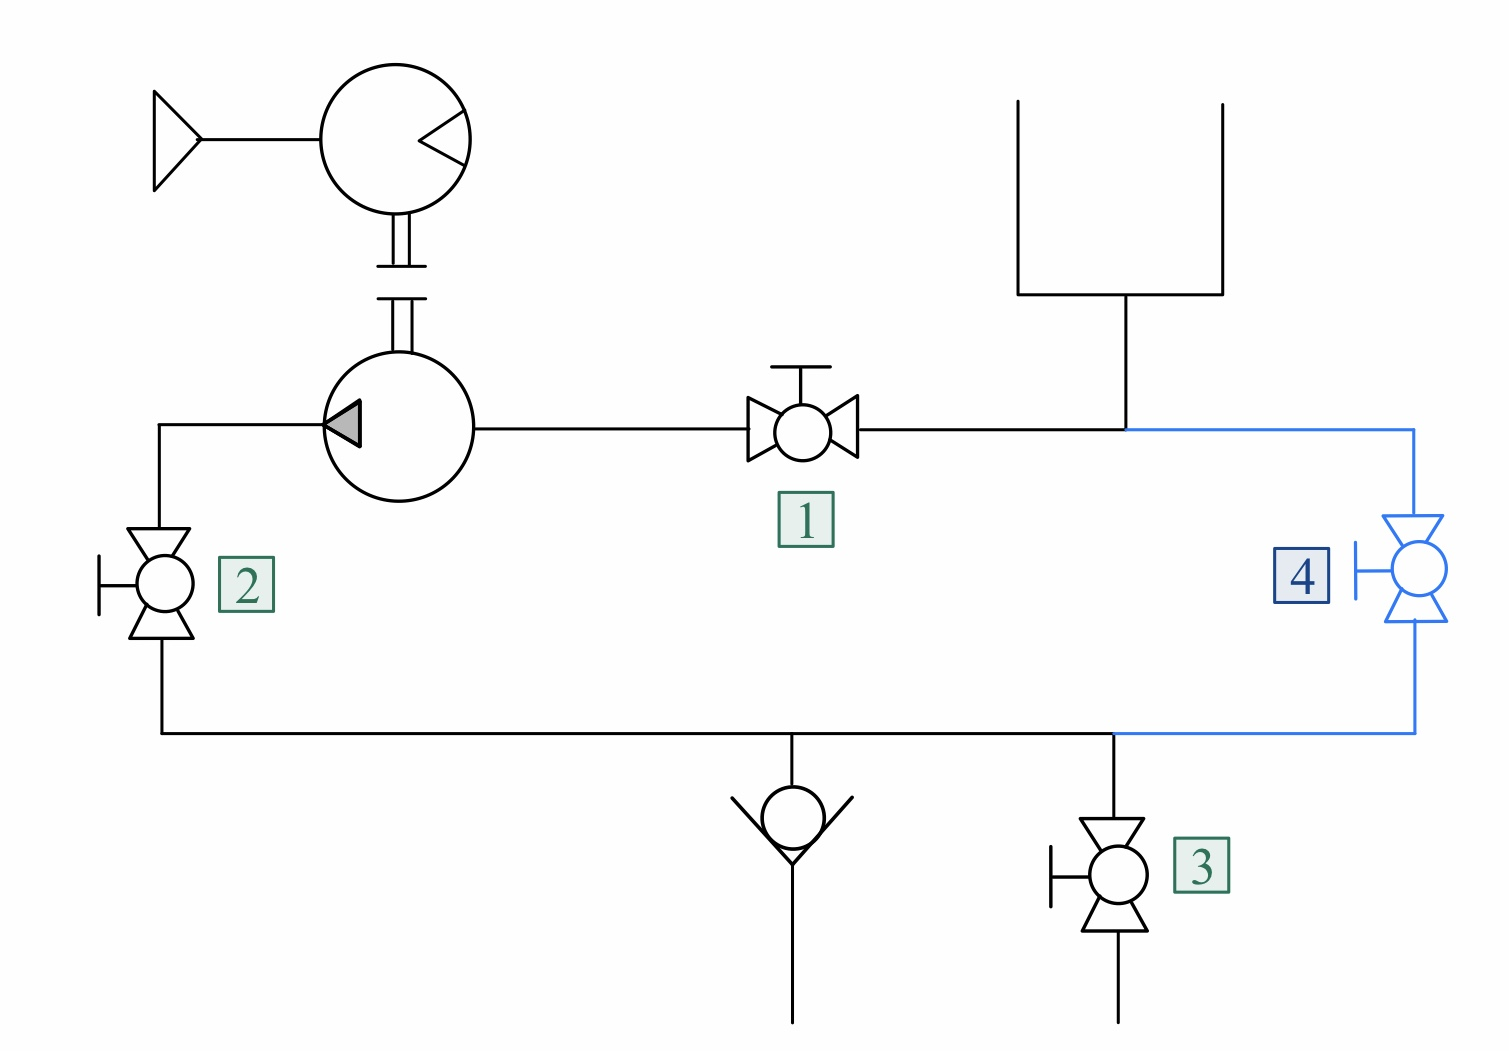
\includegraphics[width=0.5\textwidth]{figures/TestRig/TestRig2.jpg}
    \caption{Sketch of a improved test rig.}
    \label{fig:TestRig2}
\end{figure}